\section{Training and evaluation of word2vec}
\label{sec:training-and-eval-our-word2vec-impl}
In this section, we will describe training and evaluation of our word2vec model. Before we can train a word2vec model, we first have to prepare the data. For this reason, we will go over the data preprocessing choices we have made prior to training word2vec. Furthermore, we discuss the details of our own implementation of word2vec using the Skip-gram model and negative sampling, implemented using the Python programming language. At last, we cover the hyperparameter choices used to train the word2vec model and evaluate the performance of the word2vec model using analogy test data sets.

\subsection{Data preprocessing}
\label{sec:word2vec-data-preprocessing}
To train a word2vec model, one needs to have a sufficiently large data set (and thus embedding dimensionality) to yield good quality word embeddings \cite{mikolov2013b}. In the empirical experiments of \cite{mikolov2013b}, they used an internal data set based on data from Google News. Since this data set is not publicly available, we instead used dumps from \cite{WikimediaDumps} and performed a number of preprocessing steps, before training on it. In particular, we used the \textit{enwiki} (short for English Wikipedia) dump from 1st of January 2021 (20210101 on the Wikimedia pages). The dumps from Wikipedia were first downloaded and parsed using the WikiExtractor tool \cite{Wikiextractor2015}. Furthermore, we created a script using Python to merge and process output files from the WikiExtractor tool into a certain number of text files, such that we can train word2vec at ease. In order to benefit from parallel reading, we let the number of text files equal the number of CPU cores on our machine.

We then proceed by processing each Wikipedia article. In particular, we performed the following steps:
\begin{enumerate}
    \item We split each article into a list of sentences using the \path{tokenize.sent_tokenize} function from the NLTK library \cite{bird2009natural}.
    \item Then, we preprocess each sentence individually.
    \begin{enumerate}
        \item We first replace contractions in each sentence (e.g. I'll $\mapsto$ I will, you'd $\mapsto$ you would, etc.) by using the \path{contractions} pip-package \cite{contractions-2016}.
        \item Then we split the sentence into a list of words using the \path{word_tokenize} function from NLTK.
        \begin{enumerate}
            \item We convert each word in the sentence to its lower-case representation.
            \item We remove punctuation from words and create new sub-words for each word delimited by punctuation (e.g. out-of-the-box $\mapsto$ out, of, the, box).
            \item At last, we replace all numbers (including ordinal numbers) with its textual representation, using the \path{num2words} pip-package \cite{num2words2014}. For example, the number 10 becomes "ten" and the word "21st" becomes "twenty-first".
        \end{enumerate}
    \end{enumerate}
    \item With the new processed sentences, we filter out sentences that have less than \textbf{min\_word\_count} words in them.
    \item Each sentence is then appended to an output text file, separated using the newline character (i.e. \textbackslash n).
\end{enumerate}

Following, we combine common phrases of words into single tokens, where each word in the phrase is separated by an underscore, e.g. the phrase "New York" becomes "new\_york". We follow the word2phrase procedure explained in \cref{sec:learning-word-embeddings-for-phrases}. We denote the threshold parameter from word2phrase as \textbf{threshold-word2phrase}. One usually runs a couple of passes through the text data to create trigrams, four-grams or even five-grams, depending on the application at hand, and is chosen as a hyperparameter as well. We denote the number of passes through the text as \textbf{num-epochs-word2phrase}. For each pass through the data, the threshold parameter $\delta$ is decreased, although \cite{mikolov2013b} does not state how they decrease it. By inspection of the source code of word2vec, we observed that they started with a threshold of 200, then decreased it to 100 for the second and final pass. With this in mind, we introduce a threshold decay hyperparameter, denoted \textbf{threshold-decay-word2phrase}, which tells how much the threshold should be decreased for each pass.

\subsection{Implementation specifics}
To implement the word2vec model, we used Python and Tensorflow \cite{tensorflow2015-whitepaper}. In addition to this, we used the \path{numpy} \cite{2020NumPy-Array} package to work with vectors and matrices more easily. In particular, we implemented the Skip-gram model using negative sampling. To do so, we split our implementation into three main Python classes. The first class is the \path{Tokenizer}. It is responsible for converting text into word indices in vocabulary (e.g. the word "hello" $\mapsto$ 42). The second class is the \path{Word2vecSGNSModel}, which inherits the \path{tf.keras.Model} class from Tensorflow\footnote{We created the model using subclassing, as specified in \href{https://www.tensorflow.org/guide/keras/custom_layers_and_models}{this guide from Tensorflow}.}, and is the model we use to train our ANN. The third and final main class is \path{Word2vec}. It performs training using the \path{Word2vecSGNSModel} and uses \path{Tokenizer} internally to convert words into integers.

To load the data into the model, we use the \path{tf.data} API, as introduced in Tensorflow 2. The \path{tf.data} API allows us to create flexible and scalable data generators. As mentioned in \cref{sec:word2vec-data-preprocessing}, we want to train our model on dumps from Wikipedia, i.e., several gigabytes of raw text data, and the \path{tf.data} API allows us to exactly this in a quick and efficient manner. In particular, we used the \path{tf.data.TextLineDataset} class to load multiple text files in parallel and set \path{num_parallel_calls} to \path{tf.data.experimental.AUTOTUNE} wherever we could, such that we parallelize the data generation process as much as possible. We also used \path{prefetch} to prepare the data in parallel while training.

We implemented word2phrase using Python. First, we counted the uni- and bigram word occurrences, and using them, we ran the word2phrase procedure as explained in \cref{sec:learning-word-embeddings-for-phrases} by accepting bigrams into the vocabulary if the score (from \cref{eqn:word2phrase-score}) is greater than the set threshold parameter.

By implementing word2vec ourselves, we learned a few things we did not realize after reading the two original papers from Mikolov et al. \cite{mikolov2013a, mikolov2013b}:
\begin{itemize}
    \item Training on big data sets (e.g. dumps from Wikipedia) requires an efficient implementation of the data generator. We first attempted to create a data generator which loaded everything into memory, but it became clear to us that this does not scale well when we later want to test on bigger data sets.
    \item Preprocessing of data may drastically change the quality of the word embeddings.
    \item There are two embedding matrices $W$ and $W'$ corresponding to the input and output of the network. At first, we only had a single embedding matrix, for both the input and the output of the network.
\end{itemize}

\subsection{Hyperparameter choices}
\label{sec:word2vec-hyperparameter-choices}
To train the word2vec model, we base our choices of hyperparameters to the different choices used in models from \cite{mikolov2013a, mikolov2013b}. These hyperparameters can be found in \cref{table:word2vec-hyperparameter-choices}.

\begin{table}[ht]
    \centering
    \begin{tabular}{@{}ll@{}}
    \toprule
    Hyperparameter & Value\\
    \midrule
    \trcolor \textbf{min-word-count} & 5\\
    \textbf{max-vocab-size} & $\infty$ \\
    \trcolor \textbf{batch-size} & 256\\
    \textbf{num-epochs} & 5\\
    \trcolor \textbf{num-epochs-word2phrase} & 2\\
    \textbf{threshold-word2phrase} & 200\\
    \trcolor \textbf{threshold-decay-word2phrase} & 0.5\\
    \textbf{learning-rate} & 0.025\\
    \trcolor \textbf{min-learning-rate} & 0.0000025\\
    \textbf{embedding-dim} & 300\\
    \trcolor \textbf{max-window-size} & 5\\
    \textbf{num-negative-samples} & 5\\
    \trcolor \textbf{sampling-factor} & 0.00001\\
    \textbf{unigram-exponent} & 0.75\\
    \bottomrule
    \end{tabular}
    \caption{Hyperparameters used to train our word2vec model}
    \label{table:word2vec-hyperparameter-choices}
\end{table}

Similar to \cite{mikolov2013b}, we set the minimum word count to 5, i.e., we discard words that occur less than 5 times in the data we train on. In addition to this, we did not restrict the maximum vocabulary size, e.g., we let the vocabulary include any words that occur at least 5 times.

We set the number of passes for word2phrase to 2 and the initial threshold to 200, as \cite{mikolov2013b} did in their experiments. Furthermore, we set the threshold decay to 0.5 (i.e. the threshold is halved for each pass) to use a similar setup.

Neither \cite{mikolov2013a} nor \cite{mikolov2013b} stated which batch-size they used, but by inspecting the original source code\footnote{\href{https://github.com/tmikolov/word2vec/blob/e092540633572b883e25b367938b0cca2cf3c0e7/word2vec.c/\#L542}{word2vec.c at line 542 (of the original word2vec repository)}}, we concluded that they used 1 as their batch size, i.e., performing a backward pass for every forward pass in the model. We found, however, that setting the batch size to 256 to be a nice fit for our data, leading to good quality vectors and faster training.

Mikolov et al. used 1 to 4 epochs in their experiments \cite{mikolov2013a, mikolov2013b}, and in the original source code of word2vec\footnote{\href{https://github.com/tmikolov/word2vec/blob/e092540633572b883e25b367938b0cca2cf3c0e7/word2vec.c/\#L43}{word2vec.c at line 43 (of the original word2vec repository)}}, they default to 5 epochs. For this reason, we set the number of epochs to 5.

We set the initial and minimum learning rate to 0.025 and 0.000025, respectively, as noted in \cite{mikolov2013a} and the original source code of word2vec.

Furthermore, we set the embedding dimension to 300, the maximal window size to 5, the number of negative samples to 5, the sampling factor to 0.00001 and the unigram exponent to 0.75, similar to experiments from \cite{mikolov2013b}.

Using the preprocessing steps from \cref{sec:word2vec-data-preprocessing} on our data and the hyperparameters from \cref{table:word2vec-hyperparameter-choices}, we get a vocabulary size of $\sim$4.4 million words and corpus size (i.e number of words used from the \textit{enwiki} data set) of $\sim$2.3 billion words.

\subsection{Model evaluation}
We train the word2vec model using data preprocessing steps from \cref{sec:word2vec-data-preprocessing} and hyperparameters from \cref{sec:word2vec-hyperparameter-choices}. Following, we will refer to our trained word2vec model as \textit{SGNS-enwiki} (short for \textbf{S}kip-\textbf{g}ram \textbf{n}egative \textbf{s}ampling-enwiki). To show that the trained word embeddings from the SGNS-enwiki model can be used for word analogy tasks, we evaluate SGNS-enwiki using analogy test data sets. The goal of performing these tests is to show that the word embeddings are comparable to word embeddings from other models, in terms of quality.

In particular, we used three analogy test data sets, namely the Semantic-Syntactic Word Relationship test set (SSWR), the Microsoft Research Syntactic Analogies Dataset (MSR) and the Phrase Analogy Dataset (PAD). The SSWR test data set was first introduced in \cite{mikolov2013a}, consists of 8869 semantic and 10675 syntactic questions and is widely used as a test dataset. The MSR dataset was first introduced in \cite{mikolov-etal-2013-linguistic} and consists of 8000 analogy questions. To evaluate word embedding models trained on phrases (e.g. "New York Times"), \cite{mikolov2013b} introduced the Phrase Analogy Dataset (PAD). PAD consists of 3218 analogy questions. It should be noted, however, that there are other common test data sets as well, such as the Bigger analogy test set (BATS) from \cite{gladkova-etal-2016-analogy}.

We compare the results from the evaluation of our word2vec model to models from \cite{mikolov2013a, mikolov2013b, mikolov-etal-2013-linguistic, bojanowski2017enriching}. In particular, we compare to the Skip-gram models from \cite[Table 3]{mikolov2013a} and \cite[Table 6]{mikolov2013a} (denoted SG 300 and 1000 respectively), the NEG-15 model from \cite[Table 1 and 3]{mikolov2013b}, the RNN-1600 model from \cite[Table 2]{mikolov-etal-2013-linguistic} and the fastText model from \cite[Table 2]{bojanowski2017enriching}.

The results are shown in \cref{table:word2vec-eval-sswr,table:word2vec-eval-msr,table:word2vec-eval-pad}. A dash (--) denotes that the model has not been evaluated on the particular subset/data set, and \textbf{bold} values indicate the best value. Values represent accuracies and are in percentages.
\begin{table}[H]
    \centering
    \begin{tabular}{@{}cccc@{}}
    \toprule
    & \multicolumn{3}{c}{SSWR} \\ \cmidrule(l){2-4}
    \multirow{-2}{*}{Model} & Semantic & Syntactic & Average \\ \midrule
    \trcolor
    SG 300 & 55 & 59 & 57 \\
    SG 1000 & 66.1 & 65.1 & 65.6 \\
    \trcolor
    NEG-15 & 61 & 61 & 61 \\
    RNN-1600 & -- & -- & -- \\
    \trcolor
    fastText & \textbf{77.8} & \textbf{74.9} & \textbf{76} \\
    SGNS-enwiki & 65.8 & 67.3 & 66.6 \\
    \bottomrule
    \end{tabular}
    \caption{Comparison of empirical results using the SSWR word analogy test data set.}
    \label{table:word2vec-eval-sswr}
\end{table}
\begin{table}[H]
     \centering
    \begin{tabular}{@{}ccccc@{}}
    \toprule
    & \multicolumn{4}{c}{MSR} \\
    \cmidrule(l){2-5} 
    \multirow{-2}{*}{Model} & Adjectives & Nouns & Verbs & Average \\
    \midrule
    \trcolor
    SG 300 & -- & -- & -- & \textbf{56} \\
    SG 1000 & -- & -- & -- & -- \\
    \trcolor
    NEG-15 & -- & -- & -- & -- \\
    RNN-1600 & 23.9 & 29.2 & \textbf{62.2} & 39.6 \\
    \trcolor
    fastText & -- & -- & -- & -- \\
    SGNS-enwiki & \textbf{43.1} & \textbf{62.5} & 59.1 & 54.9 \\
    \bottomrule
    \end{tabular}
    \caption{Comparison of empirical results using the MSR word analogy test data set.}
    \label{table:word2vec-eval-msr}
\end{table}
\begin{table}[H]
    \centering
    \begin{tabular}{@{}cc@{}}
    \toprule
    & PAD \\
    \cmidrule(l){2-2}
    \multirow{-2}{*}{Model} & Average \\
    \midrule
    \trcolor
    SG 300 & -- \\
    SG 1000 & -- \\
    \trcolor
    NEG-15 & 42 \\
    RNN-1600 & -- \\
    \trcolor
    fastText & -- \\
    SGNS-enwiki & \textbf{53.7} \\
    \bottomrule
    \end{tabular}
    \caption{Comparison of empirical results using the PAD word analogy test data set.}
    \label{table:word2vec-eval-pad}
\end{table}

From \cref{table:word2vec-eval-sswr}, we see that our word2vec model is fairly competitive in terms of accuracy on the SSWR analogy test data set. The fastText model, however, is the most accurate model on this test data set, being approximately 10\% more accurate, on average. The same story goes for the results from the MSR test data set, as seen in \cref{table:word2vec-eval-msr}, where SGNS-enwiki performs pretty well, falling short for the SG 300 on average. Lastly, from \cref{table:word2vec-eval-pad} we see that SGNS-enwiki outperforms the NEG-15 model. Please note that we have a lot of missing data for this evaluation, as all models have not been evaluated for every (subset of the) test data set. This evaluation, however, indicates that SGNS-enwiki understands syntactic and semantic relationships between words.

To gain further insight into how the vector representations learned by SGNS-enwiki are, we inspect the nearest neighbours of words. In \cref{table:word2vec-nearest-neighbours-words} we show a sample of such comparison, using the 5 nearest neighbouring words (also some phrases) for each query word. We use cosine similarity to find the neighbouring words, excluding the query word from the search.
\begin{table}[H]
    \centering
    \begin{tabular}{@{}ll@{}}
    \toprule
    Query word & Neighbouring words \\ \midrule
    \trcolor
    Apple        & Apple Inc., Blackberry, Apple computer, OneScanner, released Xsan \\
    Phone      & Phones, mobile phone, cell phone, cellphone, phone calls \\
    \trcolor
    Water   & Fresh water, drinking water, water pumped, salinated, untreated water \\
    Sunny      & Windy, dry sunny, warm sunny, cool, Lee Hany Lee \\
    \trcolor
    Book      & Books, book entitled, Tarcher Penguin, author, foreword \\ \bottomrule
    \end{tabular}
    \caption{Nearest 5 neighbouring words for some query words, using our word2vec model.}
    \label{table:word2vec-nearest-neighbours-words}
\end{table}
From \cref{table:word2vec-nearest-neighbours-words}, we see the ability of SGNS-enwiki to identify related words to the query word.

We visualize the ability of SGNS-enwiki to identify underlying concepts of the language and relationships between them in \cref{fig:sgns-enwiki-word-to-word-relations-pca-2d}, using a 2-dimensional PCA (\cref{sec:id-estimation-lpca}) embedding of words representing countries/capitals and comparative adjectives (e.g. good $\rightarrow$ better $\rightarrow$ best). From \cref{fig:sgns-enwiki-word-to-word-relations-pca-2d}, we observe that ability of the SGNS-enwiki model to learn underlying concepts, such as what a capital means and how comparative adjectives behave. In addition to this, we also observe some clustering occurring in both plots. In particular, we observe that Scandinavian countries and capitals are more clustered to the top of the first plot (a), and words related to temperatures are more clustered to the right of plot (b).
\begin{figure}[H]
   \centering
   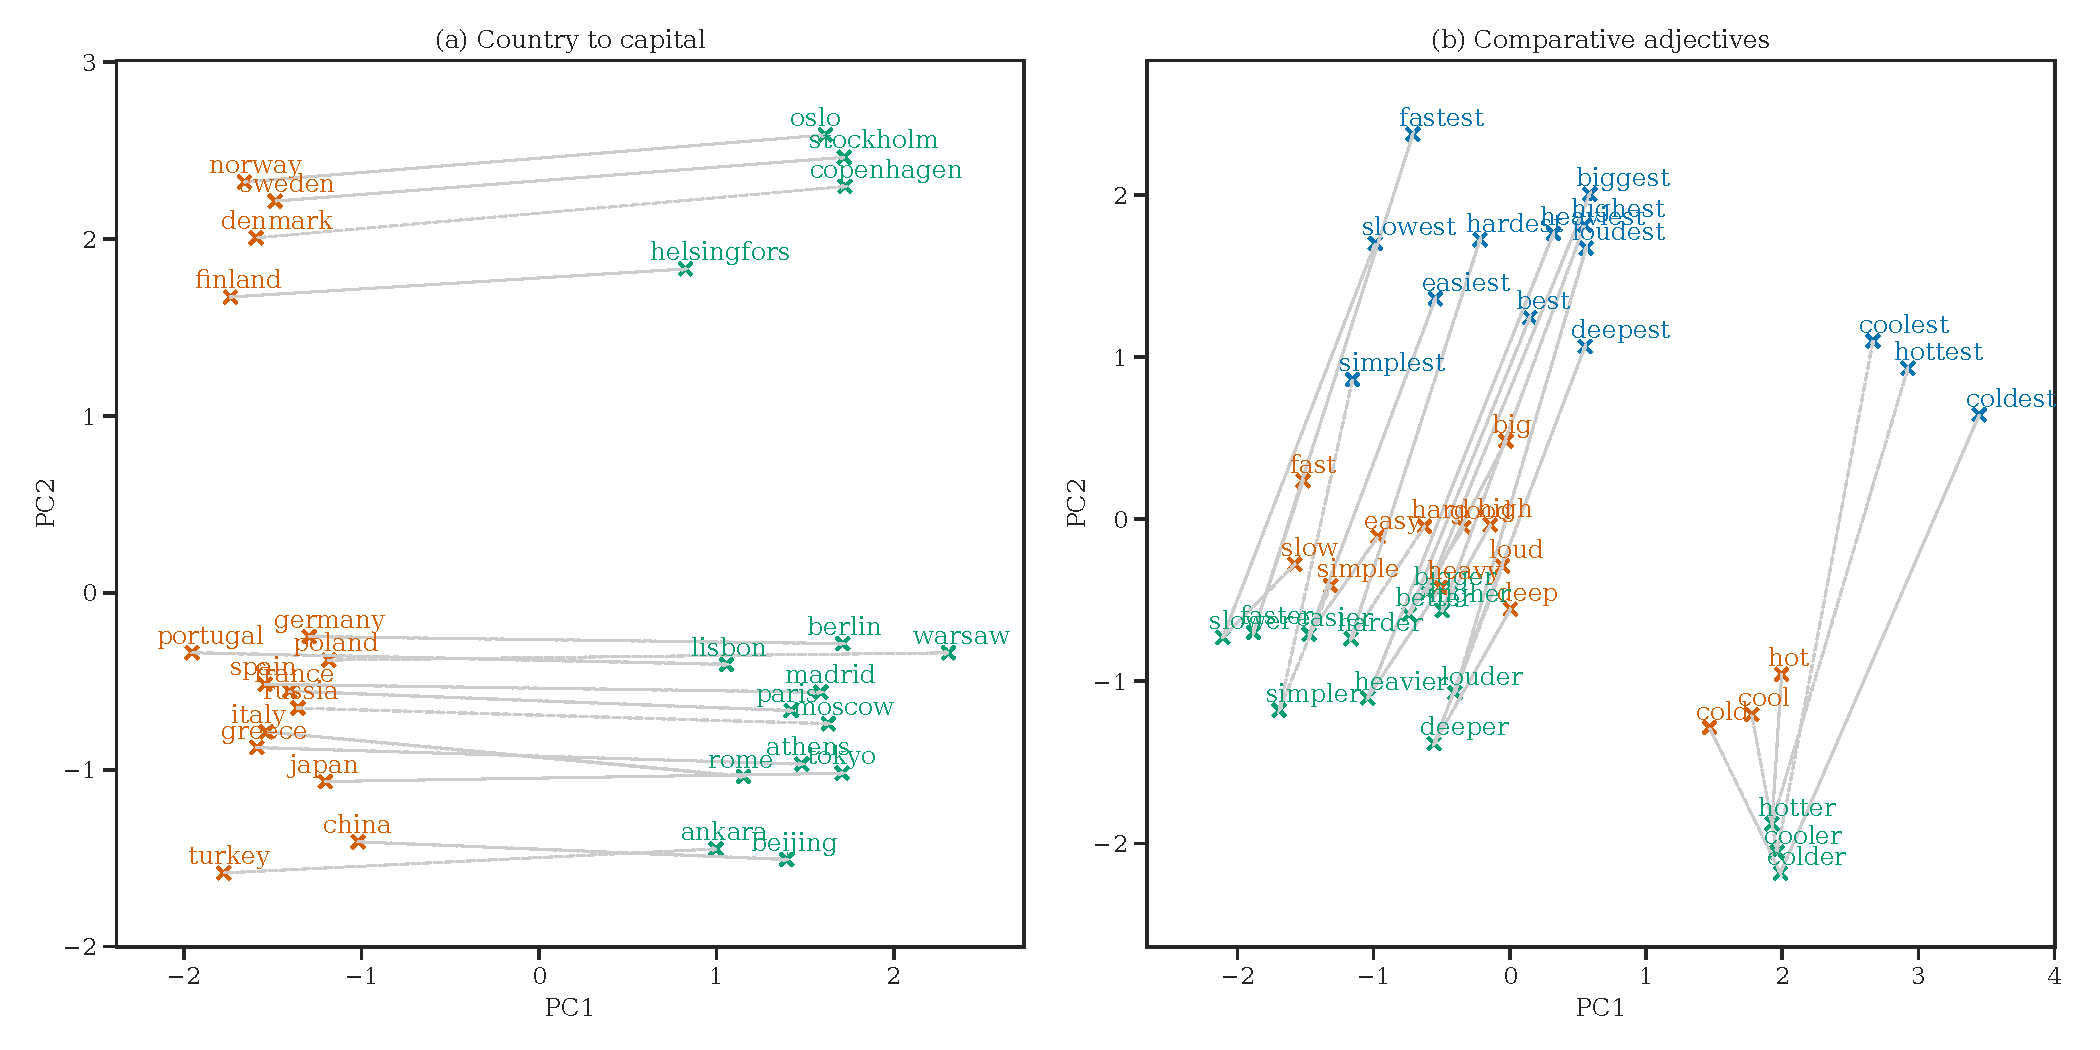
\includegraphics[width=\textwidth]{thesis/figures/word-to-word-relationships-pca-2d.pdf}
 \caption{2-dimensional PCA projection of the word embeddings of SGNS-enwiki of some countries and their capital cities (a) and comparative adjectives (b). This figure is inspired by \cite[Figure 2]{mikolov2013b}.}
 \label{fig:sgns-enwiki-word-to-word-relations-pca-2d}
\end{figure}

Due to the apparent clustering occurring in both plots from \cref{fig:sgns-enwiki-word-to-word-relations-pca-2d}, we investigate the notion of clustering further. In order to understand more about the underlying structure of the SGNS-model, we will in the next section perform cluster analysis of its word embeddings. In particular, we will use multiple clustering algorithms and internal cluster validation methods in order to find the most suitable clustering algorithm and number of clusters.